\subsection{Torque requirements}
The key outcome for single primitive optimisation is to produce physically realisable and useful constraints while minimising the required torque. It is therefore necessary to review the torque requirements and state evolution of the optimised constraints using the simulator described in Appendix \ref{chap:sim}, especially noting that the torque is only optimised for a particular initial velocity. In order to retain clarity, results in this section are limited to the 2-link compass-gait walker such that there is only a single torque.

The torque required for a particular virtual constraint to be completed over a range of initial velocities is presented in Figure \ref{fig:singleflattorque}. The result is quite predictable; the torque curves all have reasonably similar shapes (modulo numerical noise), with the footsteps at higher initial velocities requiring more torque and finishing earlier than those which started more slowly. This has the effect of contracting the curve in time but expanding it in the torque dimension. Since the shape of the torque curve is well behaved in its dependence on velocity, it is reasonable to expect near-optimality for initial velocities near the nominal.

\begin{figure}
	\begin{minipage}{0.48\textwidth}
		\centering
		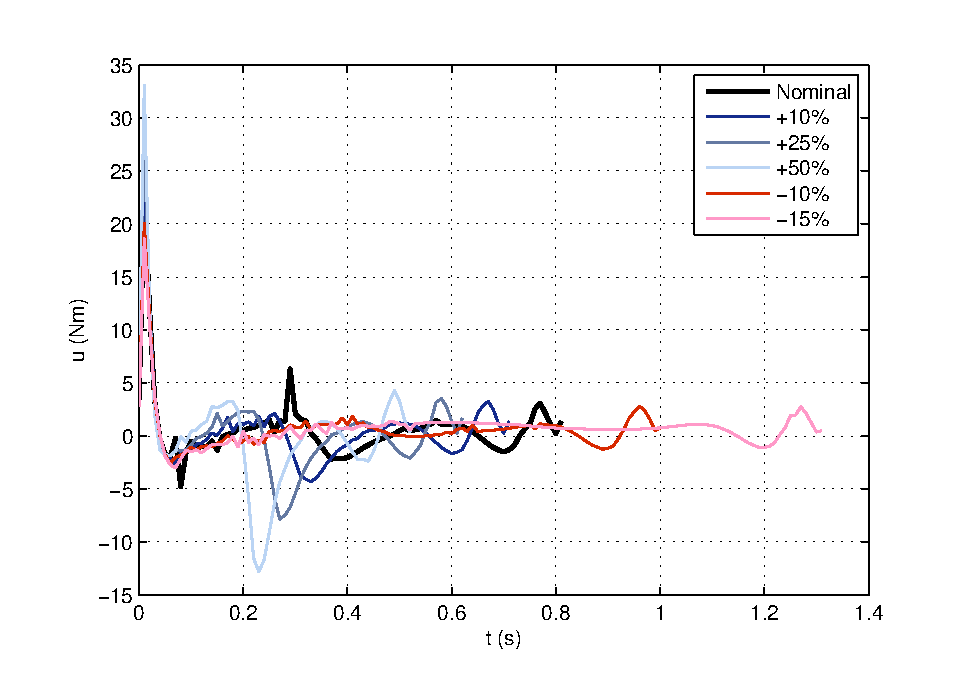
\includegraphics[width=\linewidth]{7Results/singleflattorque}
		\caption[Torque curves for differing initial velocities on flat ground]{Torque curves for different initial velocities of a virtual constraint on flat ground with $s_l=0.3$m}
		\label{fig:singleflattorque}
	\end{minipage}
	\hfill
	\begin{minipage}{0.48\textwidth}
		\centering
		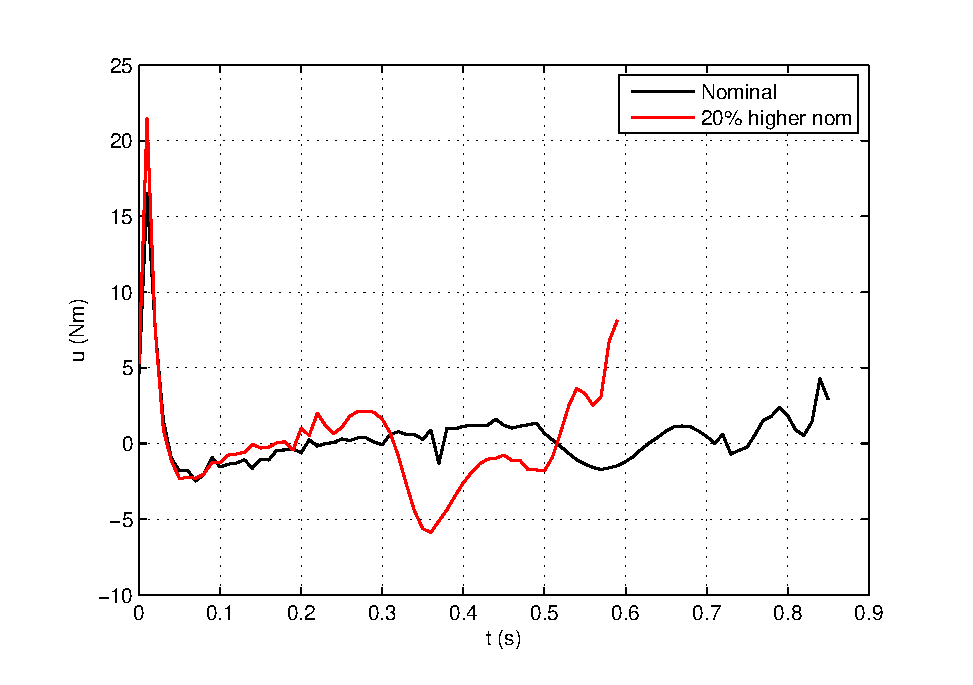
\includegraphics[width=\linewidth]{7Results/twonomvels}
		\caption[Torque curves with differing nominal velocities]{Torque curves for similar constraints with the same initial velocity but optimised for different nominal velocities}
		\label{fig:twonomvels}
	\end{minipage}
\end{figure}

An alternative method for assessing the closeness to optimality of the virtual constraints for non-nominal velocities is to optimise two VCs with the same beginning and final configurations, but differing initial velocities, and to compare the torque curves. The result of this analysis with one VC optimised using the nominal velocity definition from Section \ref{sec:optmethod}, and the other with a nominal velocity 20\% larger, is displayed in Figure \ref{fig:twonomvels}. From this plot, we observe the sensitivity in the optimisation to the initial velocity; the curves exhibit greater difference than observed in Figure \ref{fig:singleflattorque}. Even so, the curves show a somewhat similar shape, and although the optimality of the curve is clearly not maintained across a range of velocities, the torque requirements remain well behaved.

Note that the torque in these plots seems excessive; from the literature one would expect to see peak torques below 1 Nm \cite{westervelt2007feedback, collins2005efficient}. It is not clear what is causing this; the calculation of nominal torque closely matches that produced by PD control (see Figure \ref{fig:pdmatchesnom}), therefore the simulation is consistent with the model used for production of the virtual constraints. While the torque appears to be significantly higher than it should be, the actual values are not of critical importance, since this is a largely theoretical exercise given the simple model used. A more complete model will include toe-off forces which are likely to lead to significantly smaller hip torques, particularly at the initial point of the constraint, which is where we observe the largest torque.

\begin{figure}
\centering
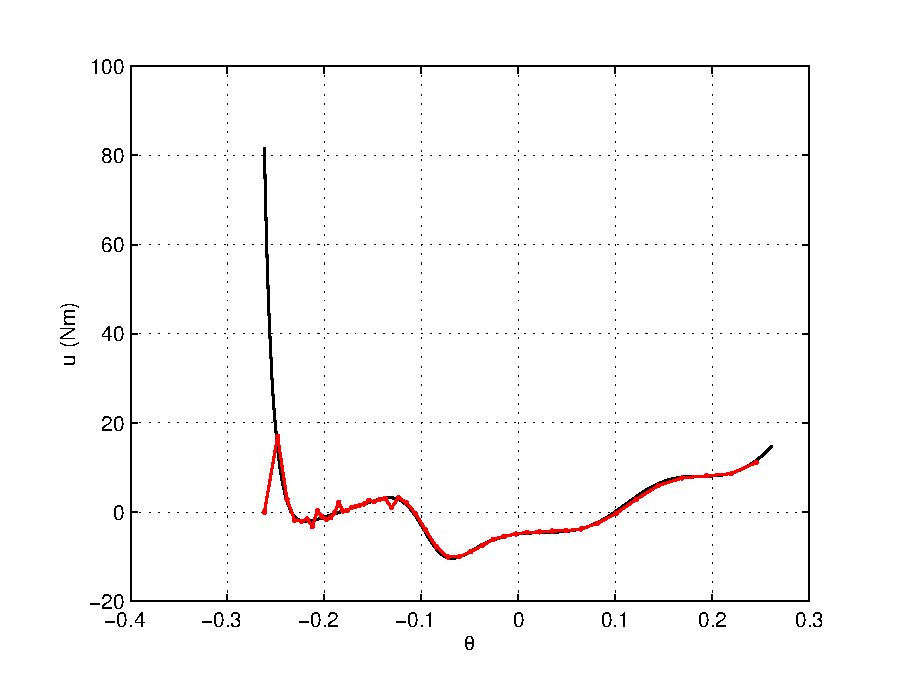
\includegraphics[width=0.5\linewidth]{7Results/pdmatchesnom}
\caption{Nominal torque and simulated PD torque for a single virtual constraint}
\label{fig:pdmatchesnom}
\end{figure}


\subsection{Kinetic energy mutations} \label{sec:reskineng}
The kinetic energy change over the virtual constraint, like the torque, is dependent on the initial velocity. In principle, this may be computed analytically, however since the analytical solution is dependent on the virtual constraint being perfectly maintained, a simulator is used such that the performance under the controller is assessed.

Table \ref{tab:vcenergy} presents the observed kinetic energy changes with varying initial velocities for a set of sample virtual constraints, each with the same initial and final configurations. Empty table cells correspond to the virtual constraint being unable to be completed due to insufficient initial velocity. A somewhat surprising result is how poorly the nominal kinetic energy mutations are realised at the nominal velocity. This is due to the numerical inaccuracies in optimising the constraint as well as those introduced by using a HZD + PD controller in the simulation. One would expect that using a transverse linearisation controller, which stabilises the velocity as well as the kinematic trajectory, would produce a more accurate realisation. 

\begin{table}
	\centering
	\begin{tabular}{ r || c | c | c | c | c | c}
		Nominal & $0.75~\dot{\theta}_{\mathrm{nom}}$ & $0.9~\dot{\theta}_{\mathrm{nom}}$ & $\dot{\theta}_{\mathrm{nom}}$ & $1.1~\dot{\theta}_{\mathrm{nom}}$ & $1.25~\dot{\theta}_{\mathrm{nom}}$ & $1.5~\dot{\theta}_{\mathrm{nom}}$ \\ \hline
		-0.05 & -0.0373 & -0.0494 & -0.0571 & -0.0695 & -0.0792 & -0.1034  \\
		0     & -0.0059 & -0.0162 & -0.0100 & -0.0198 & -0.0309 & -0.0388 \\
		0.05  &    -    &  0.0240 &  0.0096 &  0.0060 &  0.0027 & -0.0206  \\
		0.1   &    -    &    -    &  0.0473 &  0.0369 &  0.0302 &  0.0258
	\end{tabular}
	\caption[Observed kinetic energy mutations with varying initial velocity]{Observed kinetic energy mutations in joules with varying initial velocity}
	\label{tab:vcenergy}
\end{table}

Encouragingly, while there is a notable increase in the loss of kinetic energy with increasing velocity, there remains a genuine range in the kinetic energy mutations available independent of the initial velocity. A more concerning result is the apparent difficulty of adding mechanical energy to the robot through the application of hip torque over a footstep. Along with using a transverse linearisation controller, an elastic impact model and feet with some appreciable spring force and a kneed robot model should rectify this.

\subsection{Grid densities} \label{sec:numsolacc}
The optimisation of a virtual constraint is significantly dependent upon the numerical partial solution for velocity and energy. The accuracy of the numerical solution therefore limits the optimality of the constraint and the closeness to which the prescribed $\Delta$KE is achieved.

\begin{figure}[b]
	\centering
	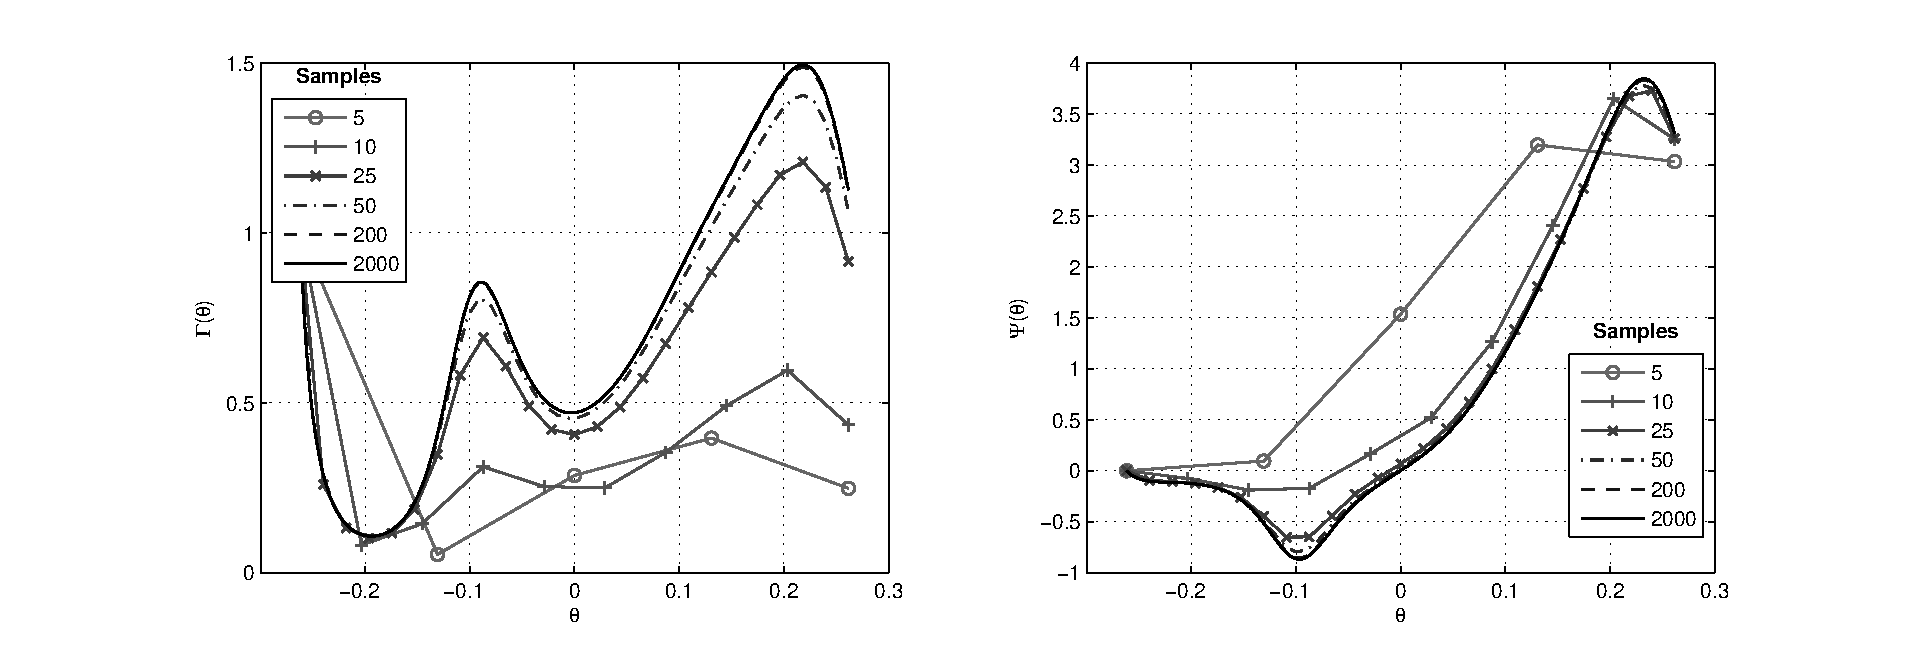
\includegraphics[width=\linewidth]{4VirtConstLib/samplingerror.eps}
	\caption{Sampling error in $\Gamma(\theta)$ and $\Psi(\theta)$}
	\label{fig:samplingerror}
\end{figure}

The partial solution (the functions $\Gamma(\theta)$ and $\Psi(\theta)$) is produced by constructing a grid of $\theta$ values, over which functions are evaluated and integrated (see Appendix \ref{app:numint}). The critical issue is that because the partial solution is generated by \textit{integration} over a grid, the accuracy of the solution is sensitive to the grid density, as shown in Figure \ref{fig:samplingerror}.

The extent of the loss of accuracy due to sampling was evaluated by optimising a self-invariant constraint on flat ground using a set number of samples $n_s$ (with sampling resolution $\epsilon_s$) with the target $\Delta$KE $=0$. A  ``ground truth'' $\Delta$KE$_{act}$ for the optimised virtual constraint was constructed using $n_s=2000$ ($\epsilon = 0.015^\circ$). The percentage error $\delta(\Delta\mathrm{KE})$ was calculated with reference to the initial kinetic energy KE$(\theta_0)$. Since the virtual constraint is self-invariant and on flat ground, $\Delta$KE $=0$ should imply $\dot{\theta}^+=\dot{\theta}^*$. The error in $\dot{\theta}^+_{act}$ was determined using a similar method as for $\Delta$KE. The results are presented in Table \ref{tab:samplingerror}.

\begin{table}
	\centering
	\begin{tabular}{ c | c || c | c || c | c | c  | c || c }
		$n_s$ & $\epsilon_s$ & $\Delta$KE$_{act}$ & $\delta(\Delta\mathrm{KE})$ & $\dot{\theta}^*_s$ & $\dot{\theta}^*_{act}$ & $\dot{\theta}^+_{act}$ & $\delta(\dot{\theta}^+)$ & CPU Time (s) \\ \hline
		5   & $6^\circ$    & -0.515 & -41.0 \% & 1.111 & 1.599 & 1.227 & -23.3 \% & 0.98 \\
		10  & $3^\circ$    & -0.262 & -22.7 \% & 1.306 & 1.533 & 1.347 & -12.1 \% & 2.15 \\
		25  & $1.2^\circ$  & 0.090  & 9.11 \%  & 1.416 & 1.417 & 1.481 & 4.50 \%  & 4.58 \\
		50  & $0.6^\circ$  & 0.014  & 1.37 \%  & 1.408 & 1.423 & 1.433 & 0.70 \%  & 6.54 \\
		200 & $0.15^\circ$ & -0.003 & -0.26 \% & 1.417 & 1.424 & 1.422 & -0.14 \% & 23.7
	\end{tabular}
	\caption[Effect of sampling error on optimisation accuracy]{Effect of sampling error on optimisation accuracy. Energy is in Joules and all velocities are in rad/s}
	\label{tab:samplingerror}
\end{table}

\begin{figure}[t]
	\begin{minipage}{0.49\linewidth}
		\centering
		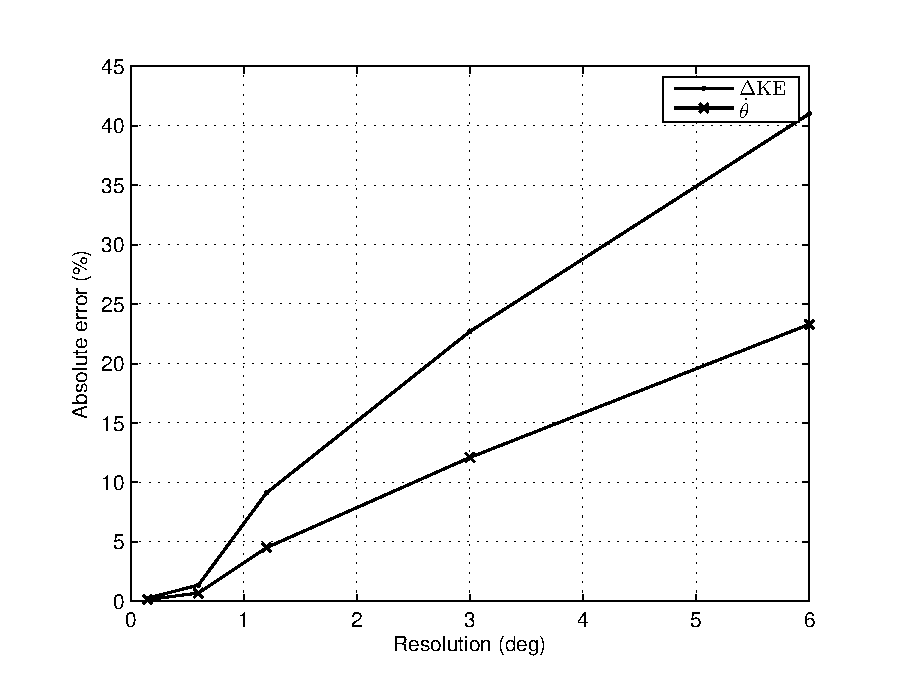
\includegraphics[width=\linewidth]{4VirtConstLib/numacc.eps}
	\end{minipage}
	\hfill
	\begin{minipage}{0.49\linewidth}
		\centering
		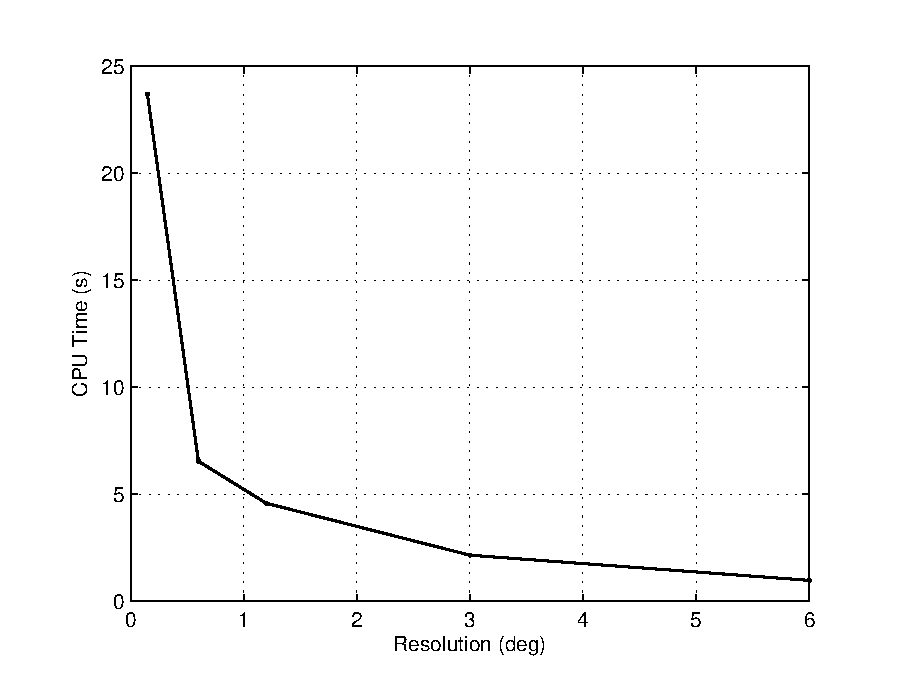
\includegraphics[width=\linewidth]{4VirtConstLib/sampleCPU.eps}
	\end{minipage}
	\caption{Sampling error and CPU time for a range of grid resolutions}
\end{figure}

From this table, we can make several key observations:
\begin{adjustwidth}{0.5cm}{}
	\begin{enumerate}[label=\bfseries Obs \arabic*, parsep=0pt]
		\item KE$(\theta^+)$ is approximately twice as sensitive to error as $\dot{\theta}^+$. This is to be expected, since KE $\propto \dot{\theta}^2$. \label{item:ke2}
		\item The solution converges to the ground truth more rapidly for small than large sampling resolutions
		\item The computation time is approximately linear in the number of samples.
		\item The error is effectively \textit{random}; there is no means of knowing \textit{a priori} if the solution is larger or smaller than the true value \label{item:randerror}
	\end{enumerate}
\end{adjustwidth}

While the importance of accuracy in the optimisation is limited, the outputs of the optimisation ($\Gamma(\theta)$ and $\Psi(\theta)$ at particular values) should be correct. It is therefore prudent to use a limited grid ($25 \leq n_s \leq 50$) for the optimisation and to then calculate the partial solution for the produced virtual constraints using much finer sampling, e.g. $n_s = 2000$. 

\subsection{Degree of the Bézier polynomial}
Increasing the degree of the Bézier curve enables finer control over the path. This is clearly favourable; however since the Bézier coefficients are the decision variables in the optimisation, increasing the degree of the polynomial increases the optimisation dimensionality. It is necessary to find a good compromise between fine control of the virtual constraint and the tractability of the optimisation problem.

Table \ref{tab:degpol} presents a comparison of a sample of degrees of polynomials. The cost $J$ for $\Delta\mathrm{KE}=-0.1,0$ and 0.1 are shown, along with the average CPU time taken to complete the optimisation. The start and end configurations are such that the virtual constraints are suited for walking on flat ground. All optimisations were performed with a grid size of 50 samples, corresponding to a grid density of 0.6$^\circ$. Note that for an accurate comparison, the cost was recalculated after the optimisation on a grid of 2000 samples.

\begin{table}
	\centering
	\begin{tabular}{c || c | c |c || c}
		Degree & $J~|~{\Delta\mathrm{KE}=-0.1}$ & $J~|~{\Delta\mathrm{KE}=0}$ & $J~|~{\Delta\mathrm{KE}=0.1}$ & Average CPU Time \\ \hline
		4  & 672 & 755 & 1109 & 0.42 s \\
		5  & 364 & 384 & 545  & 0.55 s \\
		7  & 317 & 316 & 439  & 1.56 s \\
		10 & 261 & 261 & 310  & 4.39 s \\
		15 & 427 & 427 & 427  & 10.2 s \\
		25 & 554 & 554 & 554  & 27.0 s
	\end{tabular}
	\caption{Effect of varying the degree of the Bézier polynomial in VC optimisation}
	\label{tab:degpol}
\end{table}

Figure \ref{fig:timevsdeg} shows that there is a strong quadratic fit ($R^2=0.9996$) to the CPU-time versus degree data. This should significantly motivate us to choose the minimum degree of the polynomial which achieves sufficient control over the trajectory.

\begin{figure}
\centering
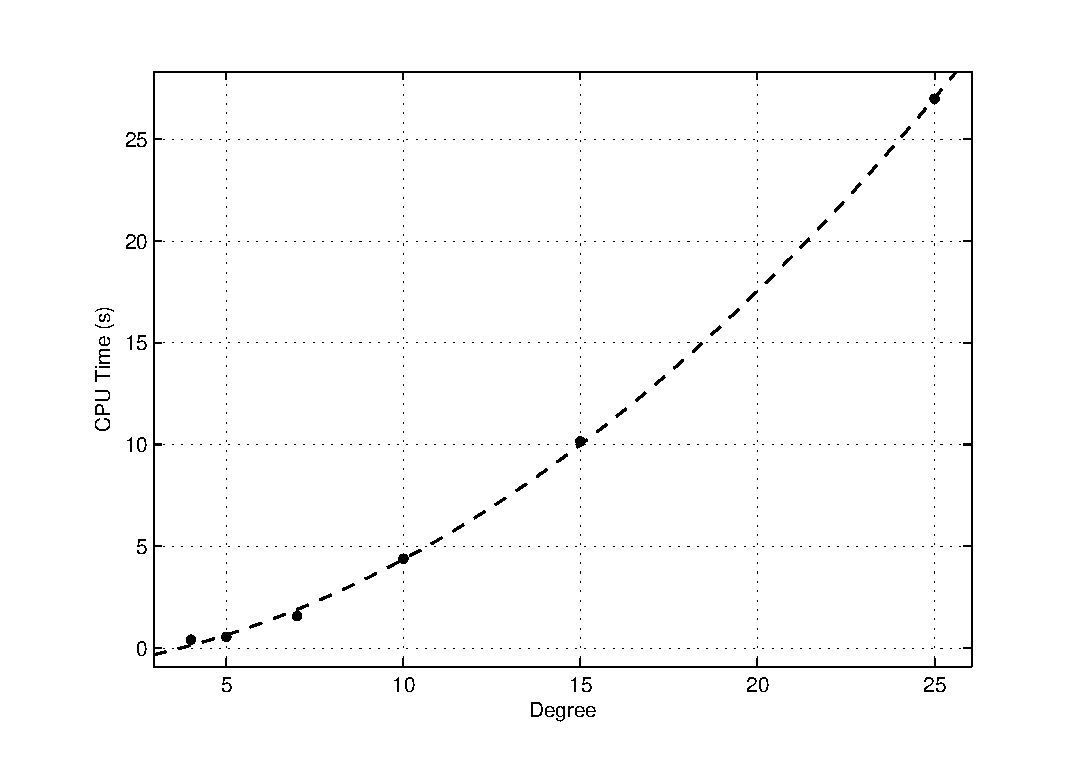
\includegraphics[width=0.6\linewidth]{7Results/timevsdeg}
\caption{Quadratic dependence of CPU time on degree of the Bézier polynomial}
\label{fig:timevsdeg}
\end{figure}

Note that increasing the Bézier degree only leads to the improvement up to a point, after which the optimisation begins fitting the numerical noise induced by the sampling error. It is also notable that in these cases, the cost for the different kinetic energy mutations is the same. This is because of the formulation of the inequality rather than equality constraint in the optimisation; the sampling error artificially deflates the cost of introducing more energy into the system. It is reasonable to expect that, even without the sampling error, the returns from a higher degree polynomial in terms of control over the shape of the virtual constraint are vanishing. The quadratic growth of the CPU time with the degree of the polynomial should also apply significant downward pressure.

\subsection{Regularisation}
As briefly discussed in Section \ref{sec:optmethod}, regularisation was used to attempt to ensure that the optimisation problem was well-posed. This was largely due to the poor behaviour of $\alpha(\theta)$ as the Bézier coefficients became large, but also to improve the convergence rates of the optimisation. It is important to recognise, however, that these gains compromise the cost function in the sense that the minimum found is no longer necessarily the minimal torque.

The effect of altering the constant $\lambda$ in Equation \ref{eqn:regcost} was assessed in terms of convergence time of the optimisation and the torque cost of the solution. Ideally, this evaluation would also include an analysis of the extent to which the optimisation avoids poor behaviour of $\alpha(\theta)$, however it is difficult to formalise this. The results of this analysis are presented in Table \ref{tab:reg}. Note that the method for producing these results was similar to that of the previous section. The virtual constraint was suited to walking on flat ground and all parameters other than the regularisation coefficient $\lambda$ were kept fixed; the degree was set to 7 and the grid size to 50.

\begin{table}
	\centering
	\begin{tabular}{c || c | c |c || c}
		$\lambda$ & $J~|~{\Delta\mathrm{KE}=-0.1}$ & $J~|~{\Delta\mathrm{KE}=0}$ & $J~|~{\Delta\mathrm{KE}=0.1}$ & Average CPU Time \\ \hline
		 1        & 317 & 316 & 439  & 1.57 s \\
		 10       & 317 & 316 & 439  & 1.46 s \\
		 100      & 316 & 315 & 438  & 1.25 s \\
		 500      & 315 & 314 & 437  & 1.06 s \\
		 $10^3$   & 316 & 316 & 437  & 1.21 s \\
		 $10^4$   & 354 & 361 & 474  & 1.30 s \\
		 $10^5$   & 470 & 530 & 691  & 1.25 s \\
		 $10^6$   & 652 & 732 & 1145  & 1.41 s \\
	\end{tabular}
	\caption{Effect of varying the regularisation constant in VC optimisation}
	\label{tab:reg}
\end{table}

\begin{figure}
\centering
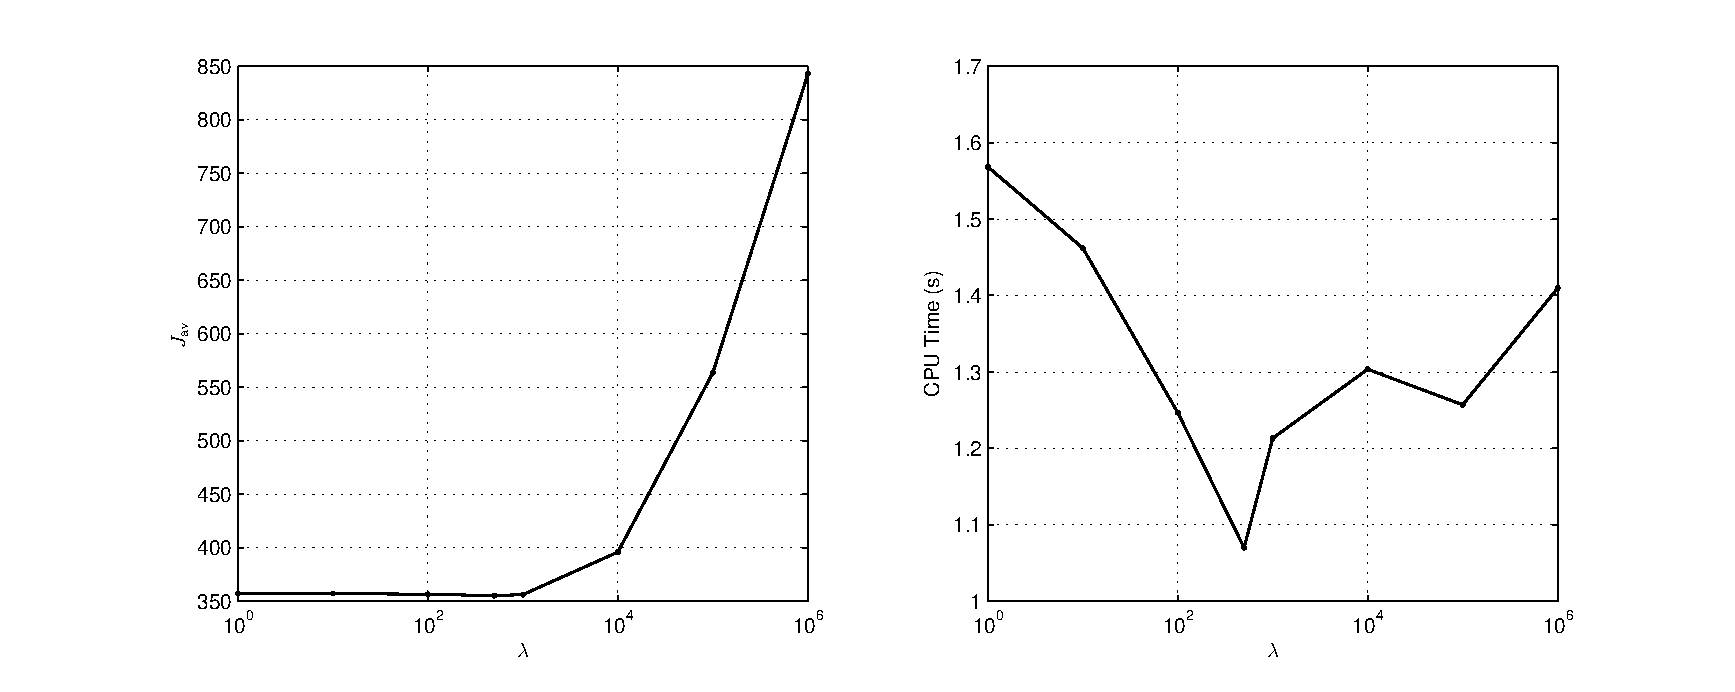
\includegraphics[width=\linewidth]{7Results/reg}
\caption{Average cost and CPU time with varying regularisation}
\label{fig:reg}
\end{figure}

It is not clear how the regularisation constant affects the convergence rate. We do not observe a clear trend of decreased computation time with increasing $\lambda$. This should be expected; we see in Figure \ref{fig:cggridtorque} that the cost is already well shaped. As discussed in Section \ref{sec:alphazerocrossing}, this is only violated where $\alpha(\theta)$ crosses zero in near-adjacent grid sections.

As expected, once the regularisation coefficient becomes comparable with $J$, the solution found by the optimisation decreases in optimality. A surprising result is the small reduction in torque cost with increasing $\lambda$ observed until $\lambda=500$. We also observe the fastest convergence at this point. It is not clear why this should be the case. Nonetheless, in this case, we do not need to make a compromise between performance and the optimality, since these appear to coexist at $\lambda\approx500$.